\vspace{0.015\textheight}
This chapter provides a description of the datasets used in this analysis. It explains the triggers used to collect data, time periods, and total integrated luminosity of the datasets. It also describes the Monte Carlo datasets used for background modeling. Furthermore, the selection of photon + jets events from data is explained in detail and the effect of the photon selection requirements is illustrated.

\section{Datasets}
\vspace{0.03\textheight}
\subsection{Data}
This analysis uses data collected from three high-\pt photon triggers. They are labeled \firstphotrig, \secondphotrig, and \thirdphotrig, where the last two digits indicate the minimum \et of the calorimeter energy required to pass that trigger. The events selected by these triggers are collected via a data stream labeled \newterm{c-stream} and the datasets are labeled with the prefix $c$. Events are taken from the photon datasets \photonDatasets, which were collected at CDF during run periods \runperiods (run range \runrange). The good run list \goodrunfile from the Photon Group is used to estimate the integrated luminosity of the analyzed data. The total integrated luminosity is \datalumAfterGoodRun after the good run selection, which excludes the first 400~\pbi of data (run range $<$190851) because it has no EM timing information to effectively remove non-collision events.

\begin{table}[hbtm]
\caption{Trigger paths for central (CEM) photons.}
\label{tab:TriggerCuts}
\centering
 \begin{tabular}{lccc}
\hline
\BUbf{Trigger Level} & \textbf{\firstphotrig} & \textbf{\secondphotrig} & \textbf{\thirdphotrig} \\
\hline
\multirow{2}{*}{\BUbf{Level 1}} & \etg{12} & \etg{12} & \etg{20} \\
& $E_{HAD}/E_{EM}<0.125$ & $E_{HAD}/E_{EM}<0.125$ & \\[2.5ex]
\multirow{3}{*}{\BUbf{Level 2}} & \etg{21} & \etg{40} & \etg{70}\\
%\multirow{3}{*}{Level 2} & \etg{21} & \etg{40} & \etg{90} (L2-JET) or \etg{70} (L2 EM) \\
& $E_{HAD}/E_{EM}<0.125$ & $E_{HAD}/E_{EM}<0.125$ & $E_{HAD}/E_{EM}<0.125$\\
%& $Had/Em<0.125$ & $Had/Em<0.125$ & $Had/Em<0.125$ (L2 EM)\\
& $E_{T}^{\mathrm{Iso}}<3$~GeV & &\\[2.5ex]
\multirow{3}{*}{\BUbf{Level 3}} & \etg{25} & \etg{50} & \etg{70}\\
& $E_{HAD}/E_{EM}<0.055$ & $E_{HAD}/E_{EM}<0.125$ & $E_{HAD}/E_{EM}<0.125$ \\
& $E_{T}^{\mathrm{Iso}}<2$~GeV & &\\
%& $Had/Em<0.055$ & $Had/Em<0.125$ (3 tower) & $Had/Em<0.125$ (3 tower)\\
\hline
\end{tabular}
\end{table}

\subsection{Monte Carlo Datasets}
Monte Carlo (MC) event samples are used for validation, cross checks, modeling the distributions of backgrounds, and deriving additional corrections. These Monte Carlo samples are generated with a leading-order (LO) MC event generator, \pythiaText~\cite{pap:PythiaManual}, and passed through the CDF detector simulation \cdfsimText (see Section~\ref{sec:cdfsim})~\cite{www:CDFSIM}. A trigger simulation is not used for these events and hence the trigger requirement is removed when Monte Carlo events are studied. This is acceptable as the triggers are 100\% efficient in the kinematic region of data being investigated. Also, the EM timing system is not simulated in generating MC events and hence not required when selecting events. All MC event samples are generated to match the instantaneous luminosity profile of data, which is run dependent. The run dependence, however, does not cover the most recent data. Hence, all MC event samples require extra corrections so that the distribution of instantaneous luminosity matches that of data.

\begin{table}[p]
\caption{Leading-order \pythiaText MC samples used to model backgrounds.}
\label{tab:MCSampleList}
\centering
\begin{tabular}{lccc}
\hline
\BUbf{MC Sample} & \BUbf{Events} & \BUbf{Cross Section} & \BUbf{Notes}\\
\hline
Inclusive $\gamma$ & 3444250 & 624$\pm$3~pb & min. $p_{T}^{\gamma}>22$~GeV/c, $k=1.4$\\%cross section $6.244\times10^{-5}$ mb\\
Inclusive Di-$\gamma$ & 11762656 & 727$\pm$3~pb & min. $p_{T}^{\gamma}>7$~GeV/c, $k=1.4$\\[1ex]
\sc{Electroweak} & & & \\
Inclusive \zee & 23323254 & 355$\pm$3~pb & $M_{ee}>20$~\massunits, $k=1.4$\\
Inclusive \zmm & 23279458 & 355$\pm$3~pb & $M_{\mu\mu}>20$~\massunits, $k=1.4$\\
Inclusive \ztt & 22930101 & 355$\pm$3~pb & $M_{\tau\tau}>30$~\massunits, $k=1.4$\\
Inclusive \wenu & 34134323 & 1960$\pm$3~pb & $k=1.4$\\
Inclusive \wmnu & 23252069 & 1960$\pm$3~pb & $k=1.4$\\
Inclusive \wtnu & 29471407 & 1960$\pm$3~pb & $k=1.4$\\
\hline
\end{tabular}
\end{table}


\section{Event Selection}\label{sec:EventSelection}
In order to select events with a prompt photon, each event is expected to pass all of the following selection rules. An event failing any one of these rules is discarded.
\vspace{-0.02\textheight}
\begin{singlespace}
\begin{enumerate}
\item{The events should have passed at least one of the three high-\pt photon triggers: \firstphotrig, \secondphotrig\ or \thirdphotrig.
}
\item{Pass the goodrun requirement: This guarantees that the event had vital detector components running during data collection and that the information collected about the event is complete and accurate.}
\item{At least one reconstructed primary vertex: Based on the number of hits in the SVX, a good reconstructed \newterm{Class 12} vertex is chosen. Class 12 vertices require 2 or more tracks with COT hits. This requirement has an efficiency of $\sim$82\% and a fake rate of $\sim$4\% for minimum bias events \cite{cdfnote:6239}. This requirement overwhelmingly rejects inelastic and minimum bias events and helps to select events originating from the hard scattering of two partons. The best vertex is chosen to be the one with the highest $\sum \pt$ of all the tracks originating from the vertex and is required to be within $|z|<60$~cm.}
\item{Photon Selection: The event needs to have a photon candidate in the central part of the detector (\etalessthan{1.1}) with \etg{30.0} that passes standard tight photon selection requirements (see Section \ref{sec:photon_identification} and Table~\ref{tab:tightAndLoosePhotonCuts}). The photon is required to be isolated from any other object in the event. There should be no tracks with large momenta pointing to the photon energy cluster in the calorimeter. The calorimeter EM timing of the photon candidate must satisfy $|\Delta t^{\gamma}| < 4.8$~ns. No muon stubs should be present within a 30\degree cone centered on the photon energy cluster. The photon candidate should fail the beam-halo selection requirements. The effect of the photon selection requirements is demonstrated in Figs.~\ref{fig:PhotonNminusOneCuts_1} and \ref{fig:PhotonNminusOneCuts_2}.}
\item{Jet Selection: The event is required to have a minimum of one jet within \etaregion{-3.0}{+3.0} with a corrected transverse energy of \etg{15} (see \refsec{sec:jet_identification}).}
\item{Jet-\met Separation: A large angular separation is required between the \met vector and the jet vectors of all jets with \etg{15.0}. This requirement, $\Delta \phi(\met - \mbox{jet})>0.4$, is applied to reject events that are subject to a large mismeasurement of jet energy, thereby improving the measurement of \met. This is a standard practice when studying events with large \met. However, this effectively causes a loss in sensitivity to any new process with moderate \met ($\sim$20--40~\etUnits), or events in which there is actual \met close to a jet. (A novel technique that removes this insensitivity and promises to discriminate fake \met from real \met has been implemented and studied extensively. It is described in Appendix~\ref{app:MetModel}.)
}
\end{enumerate}
\end{singlespace}

\begin{figure}[p]
 \centering
\subfigure[]
{ 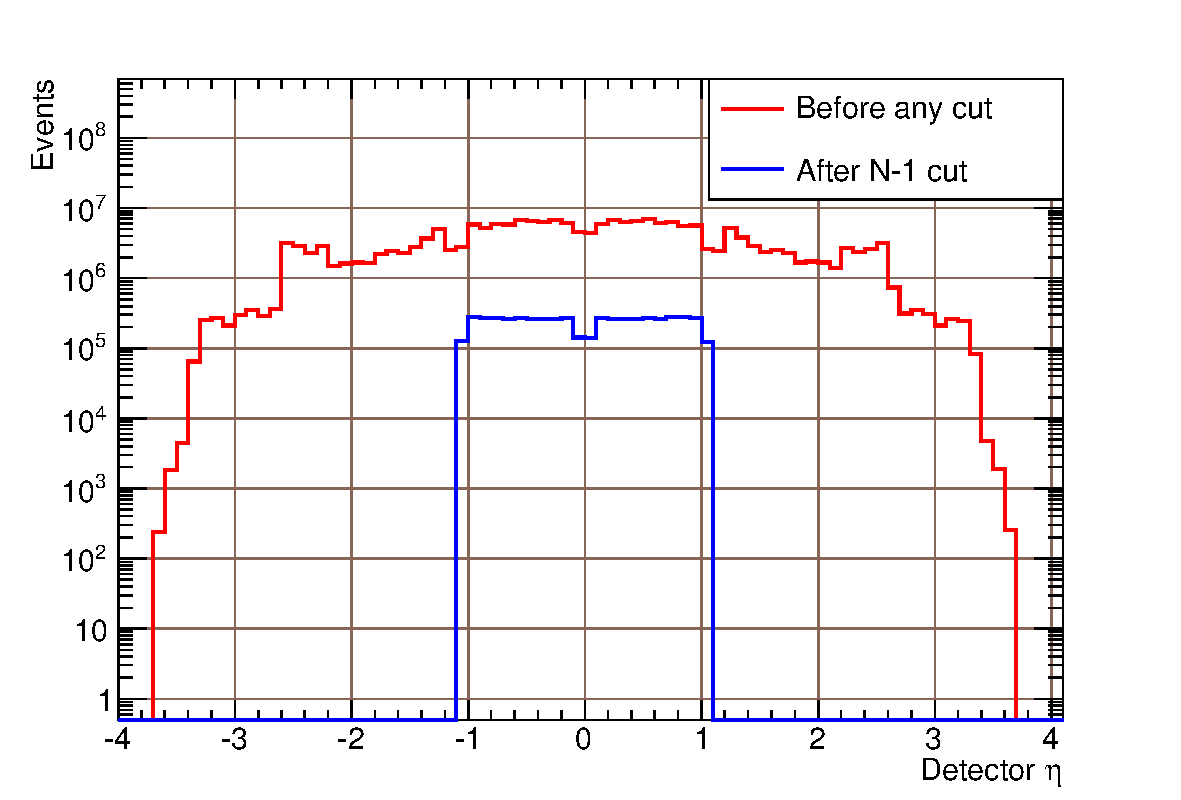
\includegraphics[scale=\phoCutsDemoHistScale,keepaspectratio=true]{./PhoCuts_Nminus1_DetEta.pdf}}
\subfigure[]
{ 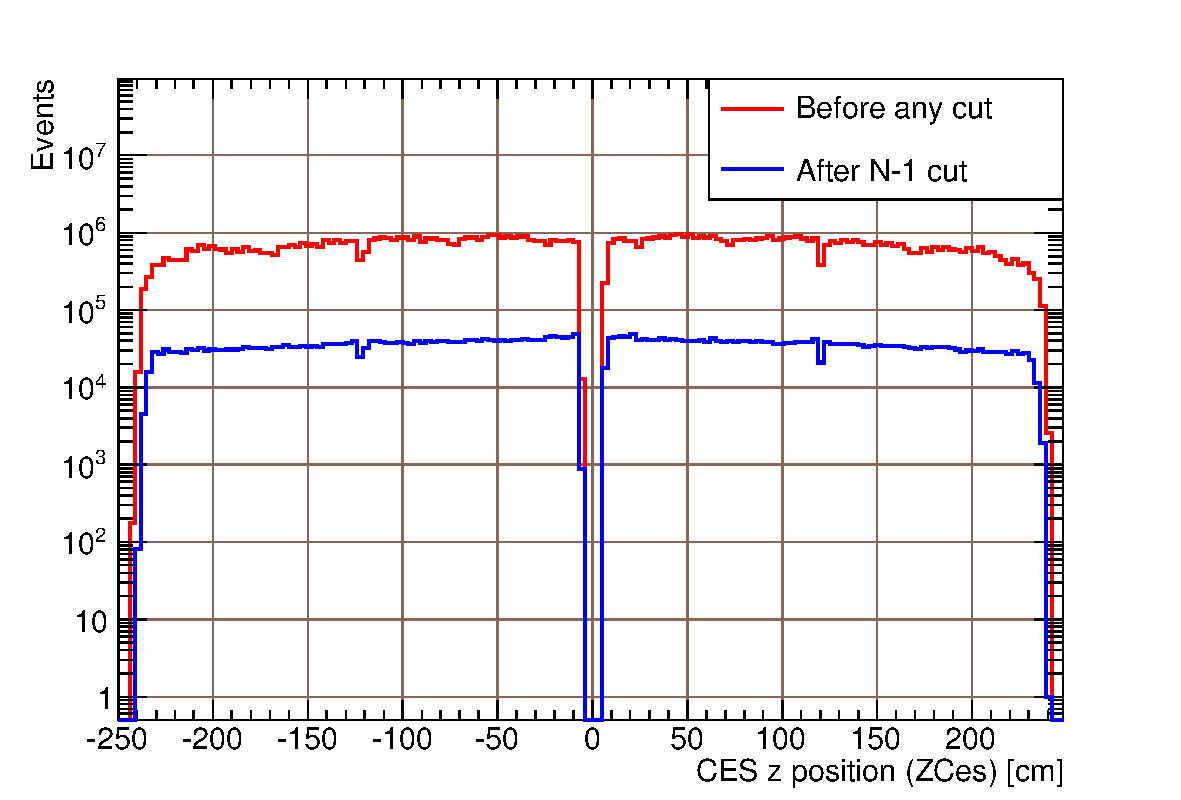
\includegraphics[scale=\phoCutsDemoHistScale,keepaspectratio=true]{./PhoCuts_Nminus1_ZCes.pdf}}
\subfigure[]
{ 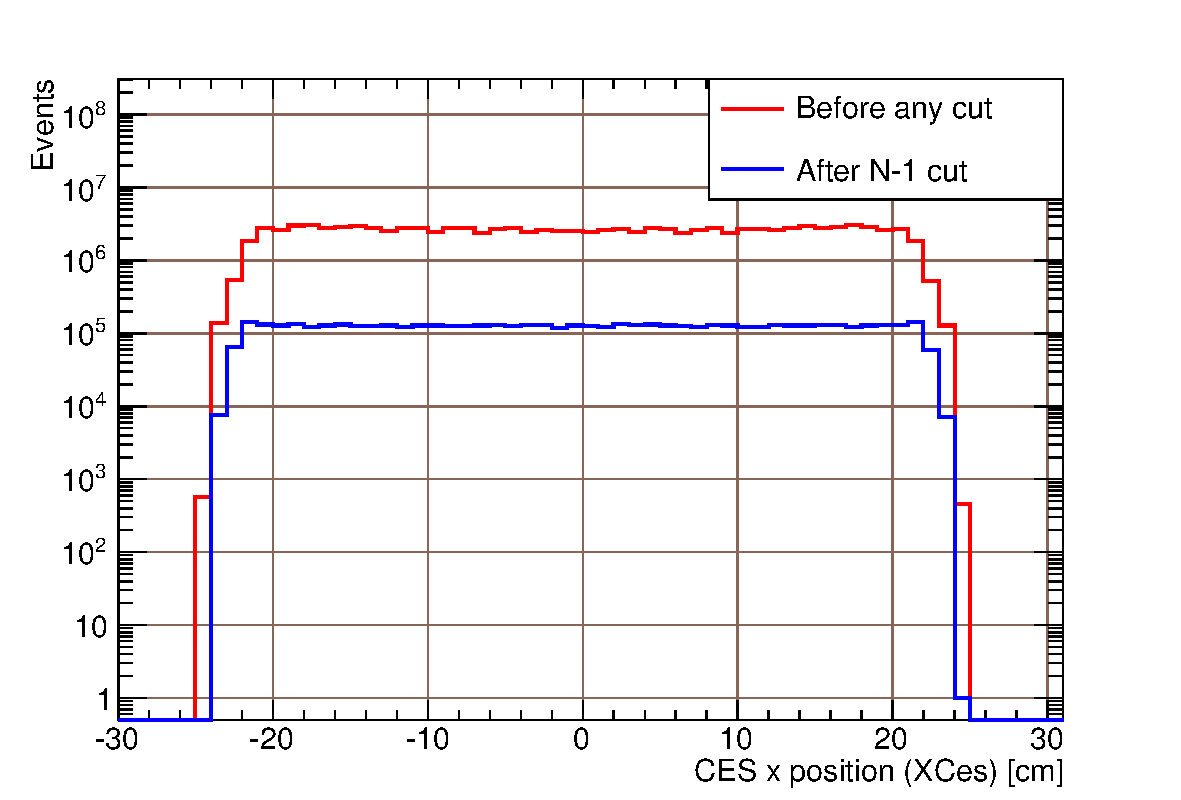
\includegraphics[scale=\phoCutsDemoHistScale,keepaspectratio=true]{./PhoCuts_Nminus1_XCes.pdf}}
\subfigure[]
{ 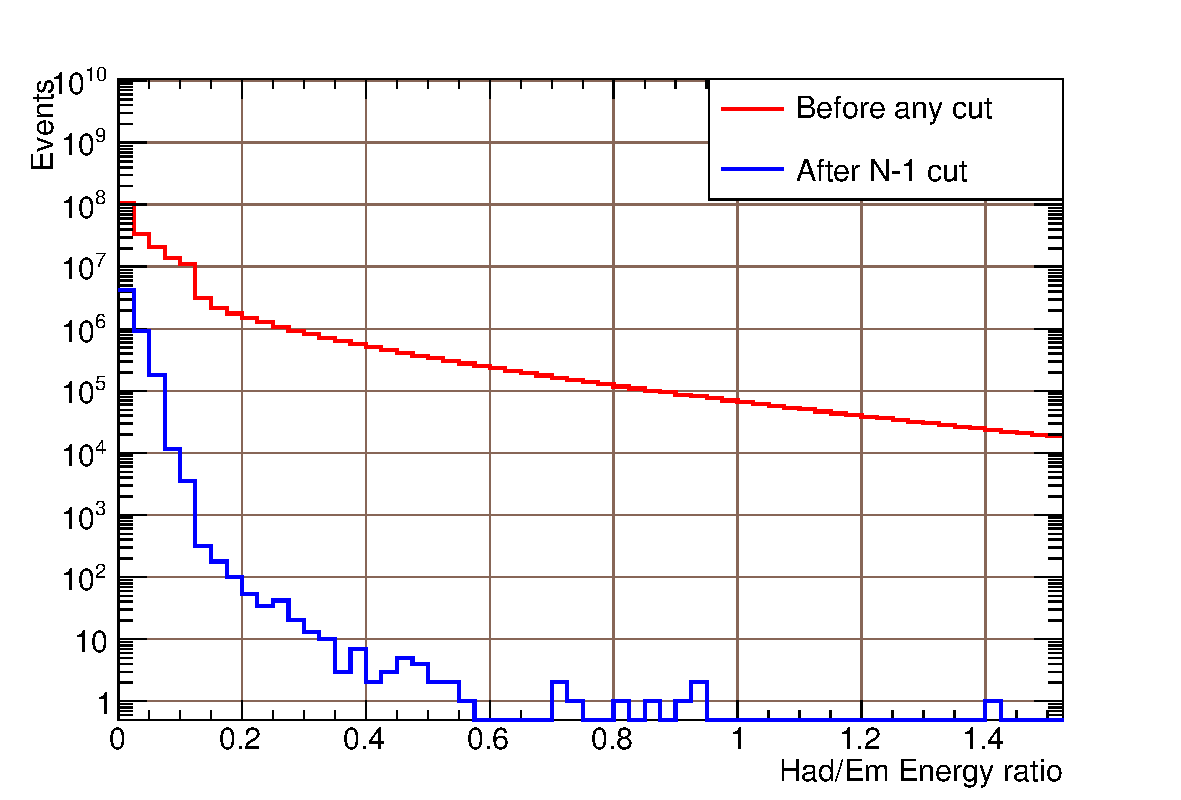
\includegraphics[scale=\phoCutsDemoHistScale,keepaspectratio=true]{./PhoCuts_Nminus1_HadEm.pdf}}
\subfigure[]
{ 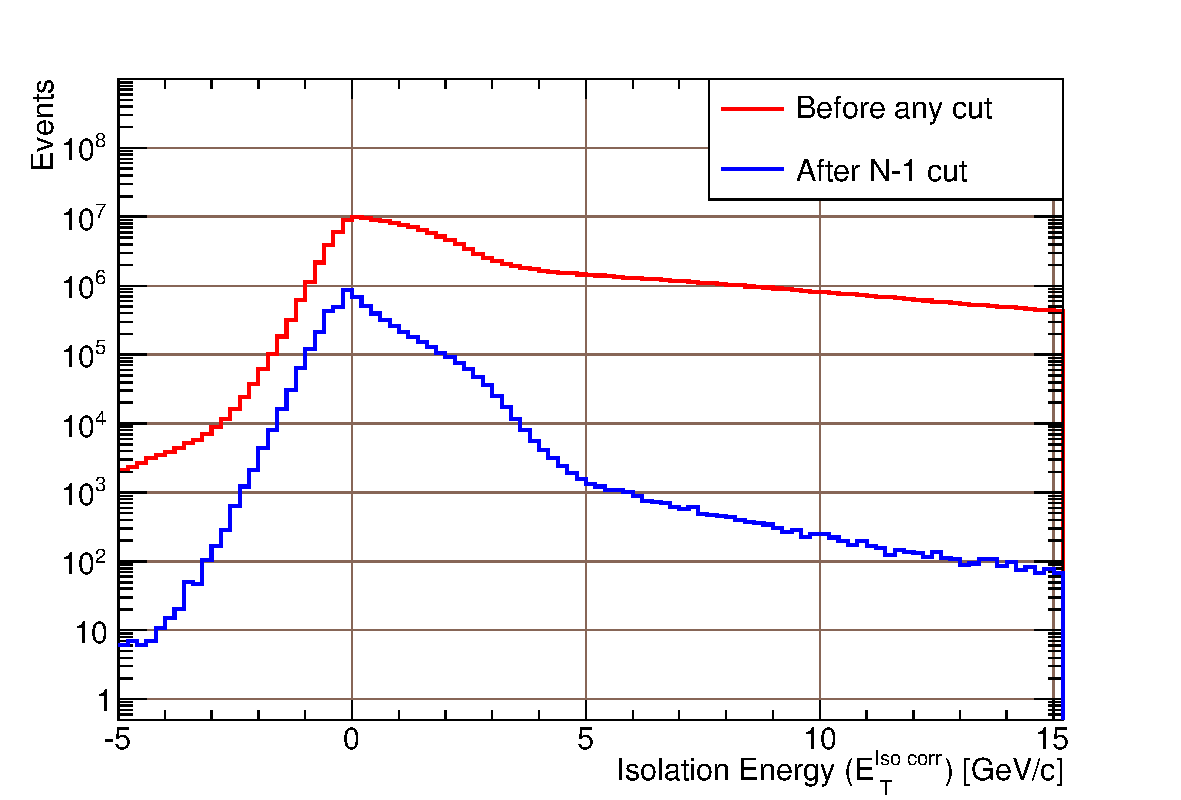
\includegraphics[scale=\phoCutsDemoHistScale,keepaspectratio=true]{./PhoCuts_Nminus1_Iso.pdf}}
\subfigure[]
{ 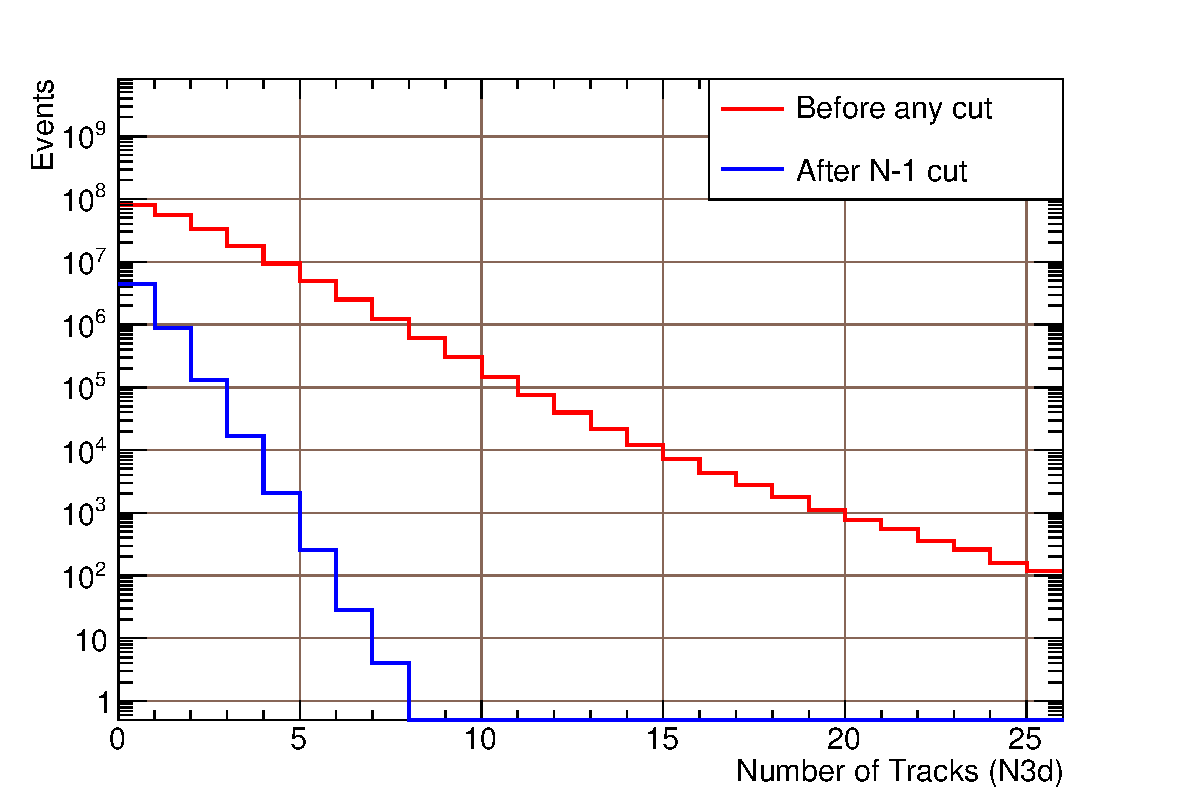
\includegraphics[scale=\phoCutsDemoHistScale,keepaspectratio=true]{./PhoCuts_Nminus1_N3d.pdf}}
 \caption{The effect of the photon selection requirements is demonstrated using $N-1$ selection requirements. For every variable to which a photon selection requirement is applied, the plot shows a distribution of the variable before any selection requirements are applied, and also after all selection requirements are applied \textit{other than} selection requirement on the variable itself.}
\label{fig:PhotonNminusOneCuts_1}
\end{figure}

\begin{figure}[p]
 \centering
\subfigure[]
{ 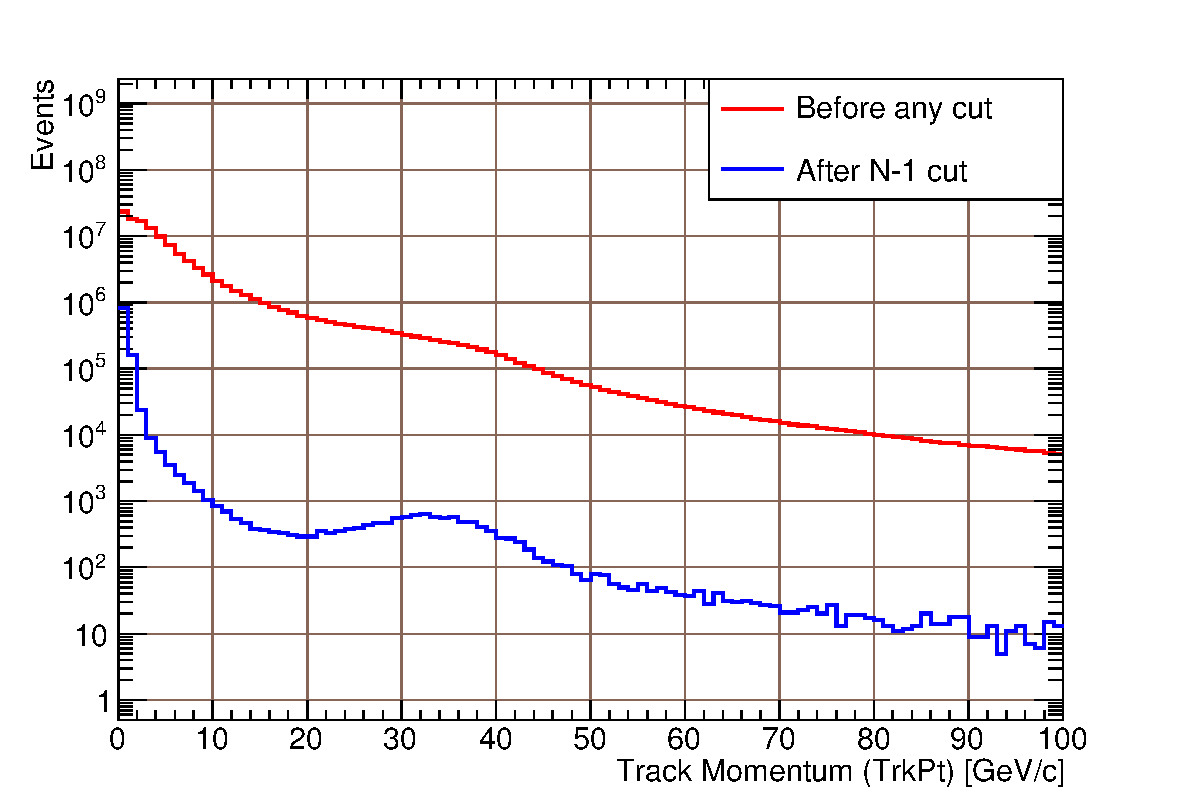
\includegraphics[scale=\phoCutsDemoHistScale,keepaspectratio=true]{./PhoCuts_Nminus1_TrkPt.pdf}}
\subfigure[]{ 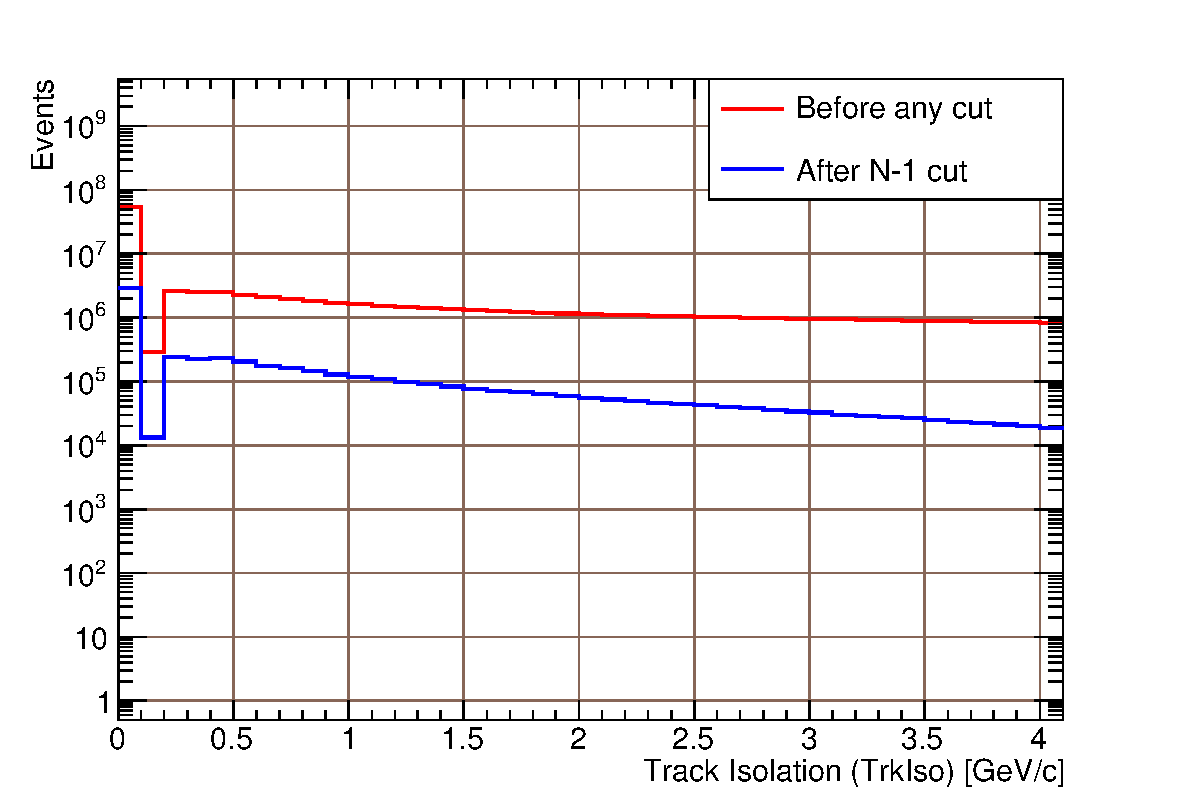
\includegraphics[scale=\phoCutsDemoHistScale,keepaspectratio=true]{./PhoCuts_Nminus1_TrkIso.pdf}}
\subfigure[]
{ 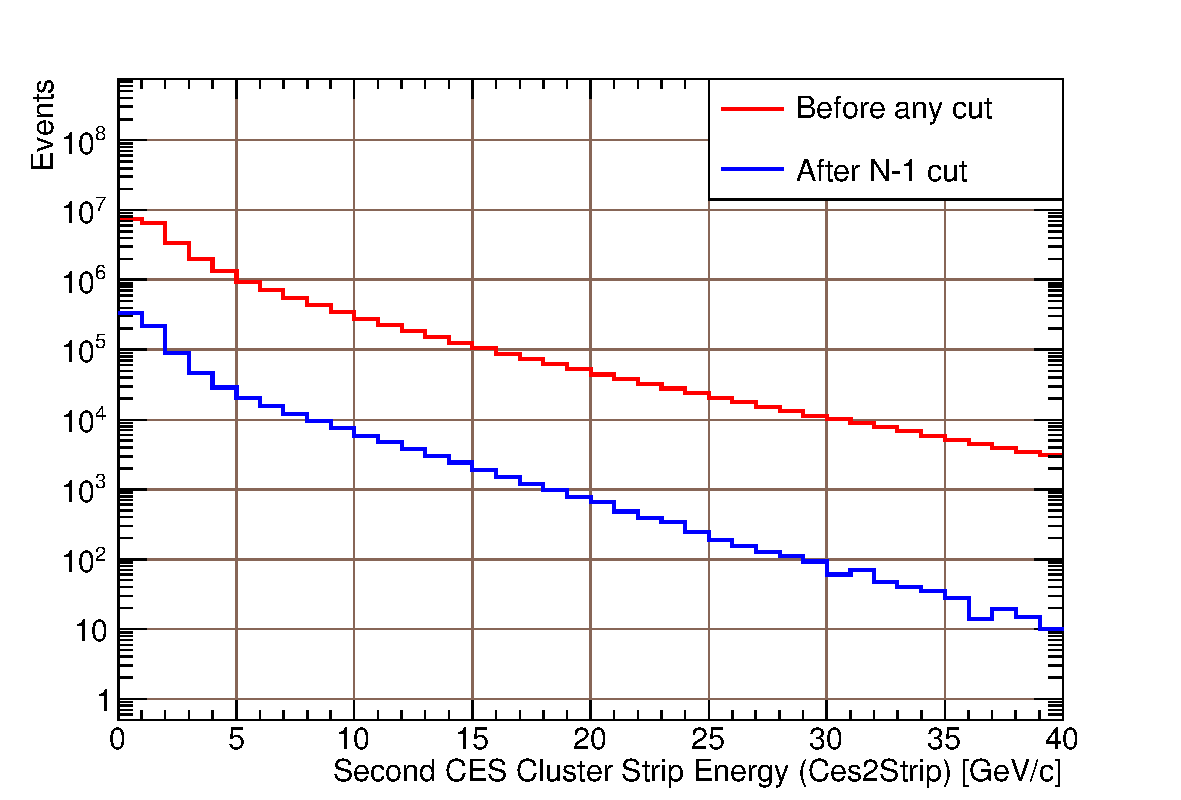
\includegraphics[scale=\phoCutsDemoHistScale,keepaspectratio=true]{./PhoCuts_Nminus1_Ces2Strip.pdf}}
\subfigure[]
{ 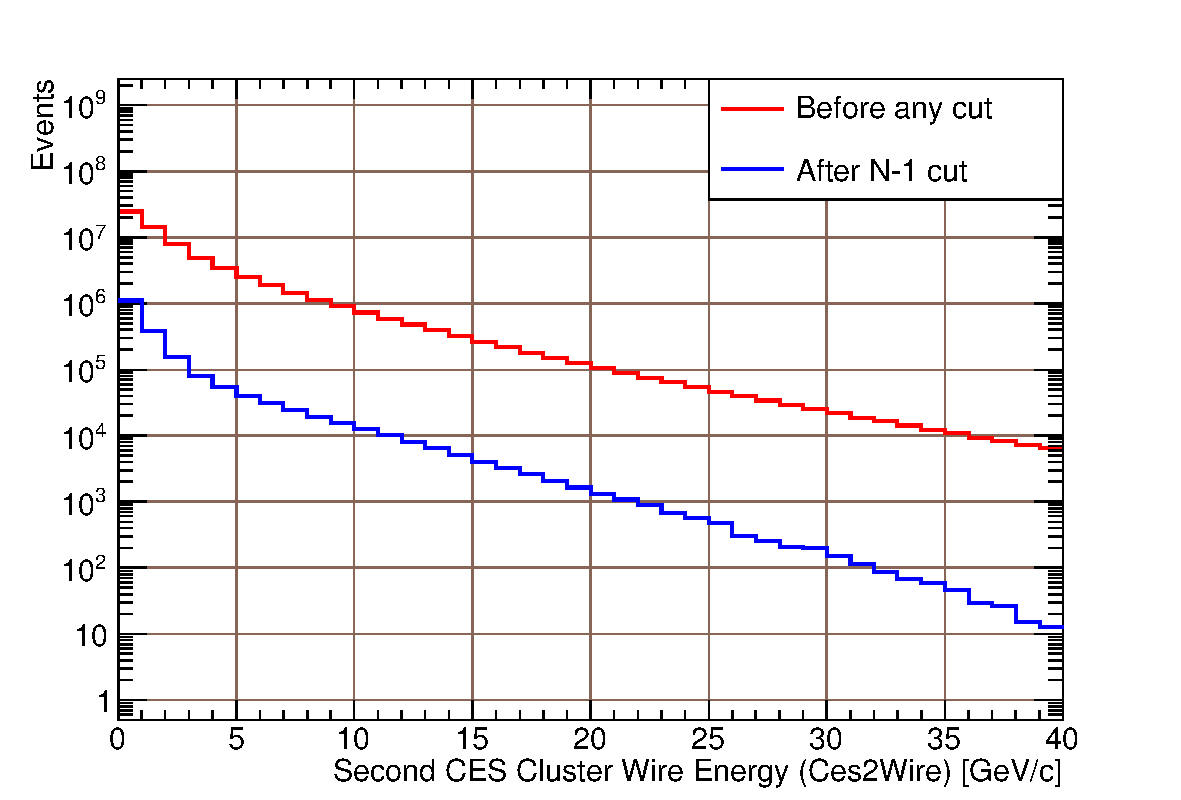
\includegraphics[scale=\phoCutsDemoHistScale,keepaspectratio=true]{./PhoCuts_Nminus1_Ces2Wire.pdf}}
\subfigure[]
{ 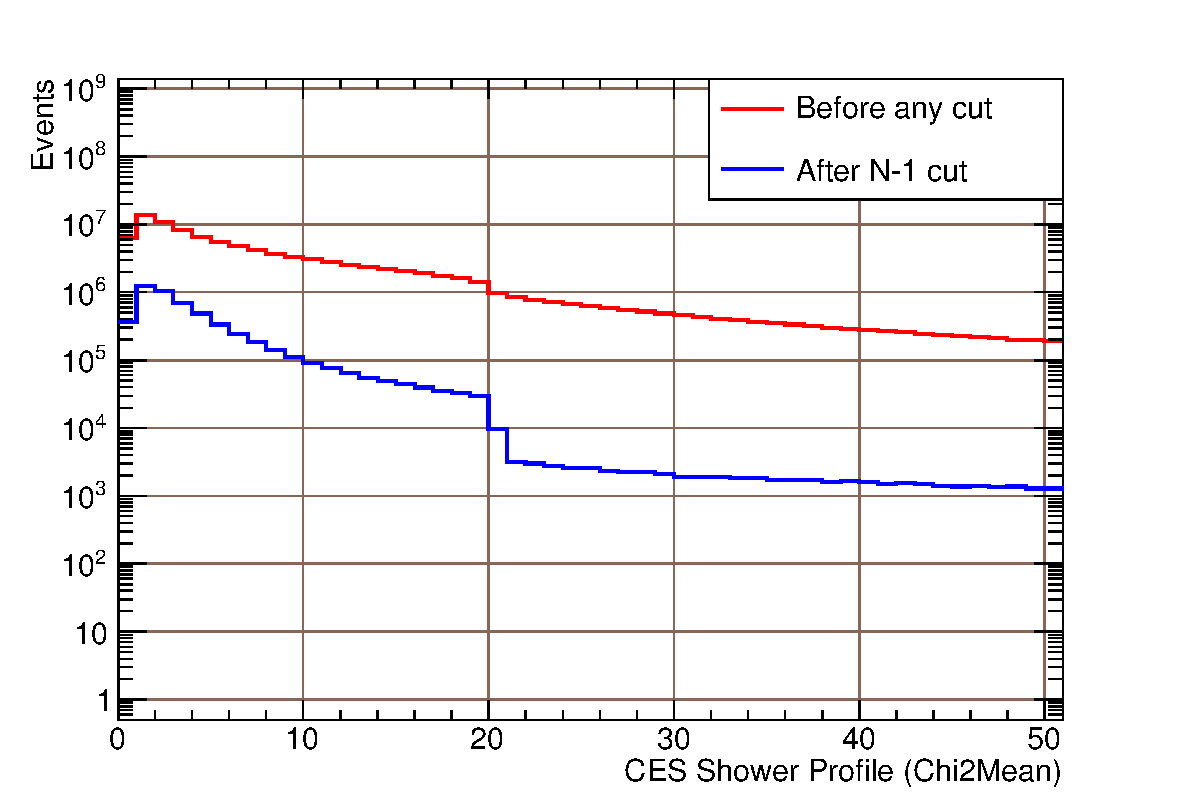
\includegraphics[scale=\phoCutsDemoHistScale,keepaspectratio=true]{./PhoCuts_Nminus1_Chi2Mean.pdf}}
% PhoCuts_Nminus1_TrkPt.pdf: 567x384 pixel, 72dpi, 20.00x13.55 cm, bb=0 0 567 384
 \caption{The effect of the photon selection requirements is demonstrated using $N-1$ selection requirements. For every variable to which a photon selection requirement is applied, the plot shows a distribution of the variable before any selection requirements are applied, and also after all selection requirements are applied \textit{other than} selection requirement on the variable itself.}
\label{fig:PhotonNminusOneCuts_2}
\end{figure}

\begin{figure}[p]
 \centering
 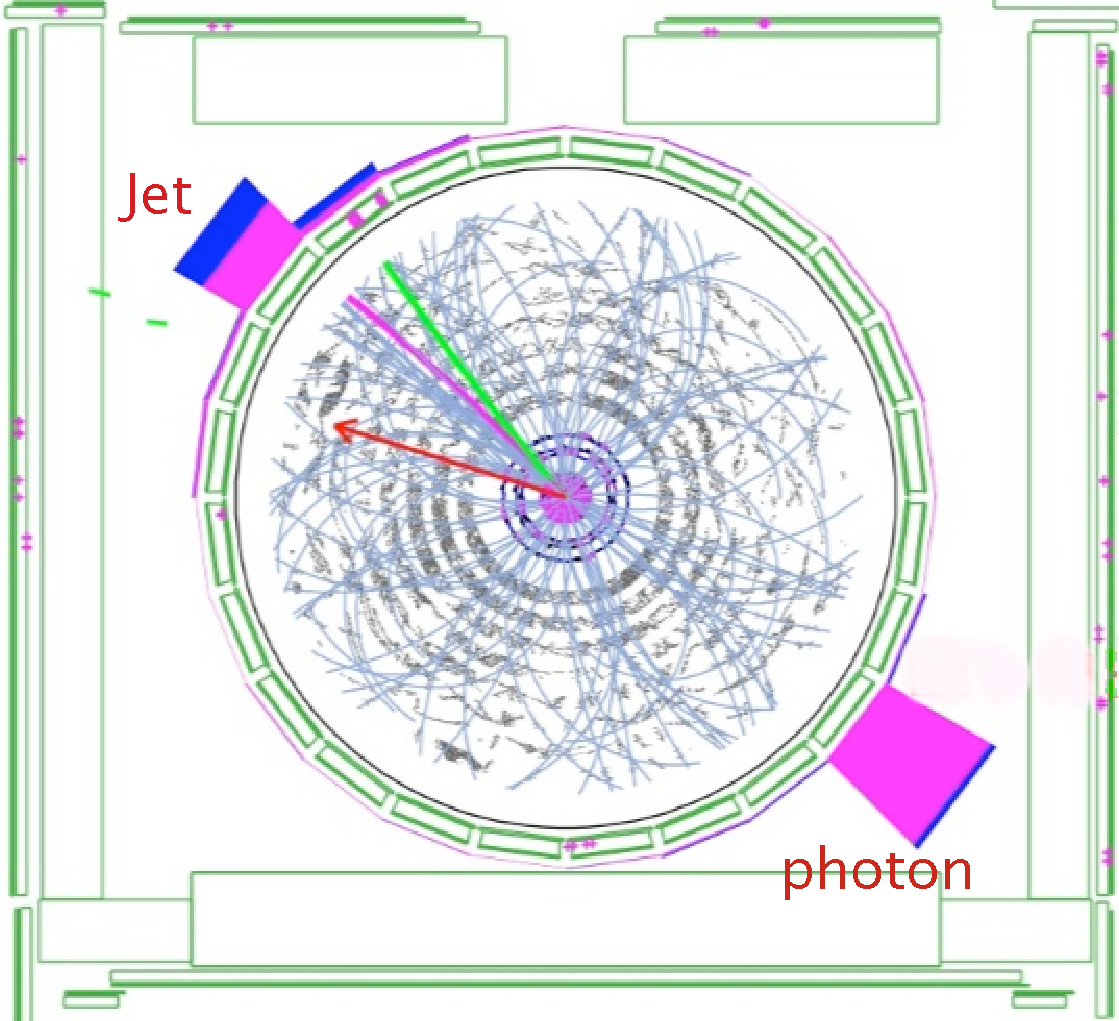
\includegraphics[scale=0.65]{./p1j_cot_edited.pdf}
 % p1j_cot_edited.pdf: 537x490 pixel, 72dpi, 18.94x17.29 cm, bb=0 0 537 490
 \caption{A photon + jet candidate event as seen in the CDF event display. There are no tracks pointing to the photon candidate and its energy is balanced by the jet. Hence, there is very little or no missing transverse energy, as indicated by the length of the red arrow.}
 \label{fig:pj1_EvtDisplay}
\end{figure}

These selection requirements are summarized in Table~\ref{tab:SignalSelection}, and Fig.~\ref{fig:pj1_EvtDisplay} shows a photon + jets candidate event as seen in the CDF event display. After the leading photon is identified in an event, other objects are treated as jets; however, extra EM objects in the event (if any) are identified using loose photon selection requirements (Table~\ref{tab:tightAndLoosePhotonCuts}) and standard loose electron selection requirements (Tables~\ref{tab:StdLooseCentalEleID} and \ref{tab:StdLoosePlugEleID}) to avoid over-correcting them by applying jet energy corrections (see Section \ref{sec:jet_identification}). Here, the standard loose electron selection requirements are used instead of photon-like electron selection requirements because they are more efficient in identifying electrons.

\begin{table}[p]
\caption{Summary of data event selection.}
\label{tab:SignalSelection}
\centering
 \begin{tabular}{cc}
\hline
\BUbf{Selection Variable} & \BUbf{Requirement}\\
\hline
Goodrun & Pass\\[1ex]
\multirow{2}{*}{Trigger} & Pass any one of the triggers\\
& \firstphotrig, \secondphotrig, \thirdphotrig. \\[1ex]
Primary Vertices & $\geq 1$ and its $z$ position $|z|<60$~cm\\[1ex]
\sc{Photon Selection} & $E_{T}^{\gamma} > 30$~\etUnits, $|\eta_{detector}^{\gamma}|<1.1$\\
& Pass tight photon\\
& selection requirements (see Table~\ref{tab:tightAndLoosePhotonCuts})\\[2ex]
EM timing & $|\Delta t^{\gamma}|<4.8$~ns\\
Tracks (Phoenix) & No phoenix tracks\\
Muon stubs & 0 (No muon stubs)\\
Beam halo selection requirements & Fail\\[2ex]
\sc{Jet Selection} & $\geq 1$ jet with $E_{T}^{jet} > 15$~\etUnits, $\eta_{detector}^{jet}|< 3.0$\\
Jet--\met separation & $\Delta \phi(\met - \mathrm{jet})>0.4$\\
\hline
 \end{tabular}
\end{table}

This study is performed with inclusive \phoonejet and \photwojet data samples. In the \photwojet data sample, a second jet is required with the same jet selection criteria applied to the first jet. The kinematic quantities measured for the \phoonejet sample are photon \et ($E_{T}^{\gamma}$), leading jet ($E_{T}^{jet}$), total energy in the event ($H_{T}$), number of jets with \etg{15}, invariant mass of the photon and leading jet, and the missing transverse energy. In addition, in the \photwojet event sample, the invariant mass of the photon + two leading jets and the invariant mass of the two leading jets are measured. In order to gain a higher sensitivity and increase the probability of discovering new physics beyond the SM, subsamples containing \phoonejet + \met and \photwojet + \met, where \met$>$~20~\etUnits, are also studied. The same kinematic quantities measured in the \phoonejet and \photwojet samples are measured in these subsamples.

\begin{table}[p]
\caption{Selection of photon + jet events from data. The selection requirements are applied in the listed order. After each selection requirement is applied, the number of remaining events is given.}
\label{tab:gjet_count}
\centering
\begin{tabular}{lr}
\hline
\BUbf{Selection Requirement} & \BUbf{Events Passed}\\
\hline
Total data events & 200711604\\
Run number is in the goodrun list & 180069651\\
Pass any of the photon triggers & 178962163\\
Number of primary vertices $\geq 1$ & 174873113 \\
Primary vertex $z$ position, $z<60$~cm & 174873113\\
{\sc Photon Selection}\\
\quad Photon with $E_{T}>30$~\etUnits & 112304018\\
\quad Photon satisfying tight photon selection requirements & 9903155\\
\quad Not PMT spike & 9896480\\
\quad $|\Delta t^{\gamma}|<4.8$~ns (cosmic veto)& 9784532\\
\quad No muons stubs in 30\degree cone (cosmic veto)& 9405230\\
\quad No tracks (lepton-veto)& 9022377\\
\quad Fail beam halo selection requirements (beam halo veto) & 7385321\\
{\sc Jet Selection}\\
\quad $\geq 1$ jet with $E_{T}>15$~\etUnits & 6576636\\
\quad All jets are away from the \met vector & 4883544\\
{\sc \met Selection}\\
\quad \met$>20$~\etUnits & 134155\\
\hline
\end{tabular}
\end{table}